% Template for reports for the seminar 
% "Domain-specific architectures for Deep Neural Networks", 
% summer semester 2020 
%

\documentclass[11pt,twoside]{article}

\usepackage{url}
\usepackage[english]{babel}
\usepackage[T1]{fontenc}
\usepackage[utf8]{inputenc}
\usepackage{times}

\usepackage[a4paper,left=2.5cm,right=2.5cm,top=3cm,bottom=2.5cm]{geometry}
\usepackage{graphicx}
\usepackage{paralist}
\usepackage{fancyhdr}
\usepackage{lastpage}
\usepackage{amssymb,amsmath}

\pagestyle{fancy}
\fancyhead{}
\fancyhead[LE]{ \slshape \participant}
\fancyhead[LO]{}
\fancyhead[RE]{}
\fancyhead[RO]{ \slshape \topic}
\fancyfoot[C]{page \thepage \hspace*{0pt} / \pageref{LastPage}}



%%%%%%%%%%%%%%%%%%%%%%%%%%%%%%%%%%%%%%%%%%%%%%%%%%%%%%%%%%%%%%%%%%%%%%%%%%%%%%
%%%%%%%%% configure these settings and you are good to go %%%%%%%%%%%%%%%%%%%%
%%%%%%%%%%%%%%%%%%%%%%%%%%%%%%%%%%%%%%%%%%%%%%%%%%%%%%%%%%%%%%%%%%%%%%%%%%%%%%
\newcommand{\participant}{Varun Maitreya Eranki}
\newcommand{\affiliation}{Paderborn University}
\urldef{\emailaddress}\url{varune@mail.uni-paderborn.de}
\newcommand{\topic}{Spiking Neural Networks - IBM TrueNorth}
\newcommand{\submissiondate}{\today}


\begin{document}

\title{\topic}
\author{\Large{\participant}\\ \affiliation \\ {\small \emailaddress}}
\date{\submissiondate}
\maketitle
\thispagestyle{empty}


\begin{abstract}
Human Brain is the most complicated, and important organ in the human body. It is fascinating to understand, how it functions with an interconnected network of billions of neurons. It is super-efficient and fast in real-world tasks and consumes 20 W of power \cite{hsu2009much, modha2017introducing}. Can computers reach such efficiency? Scientists at IBM attempted to solve this question over the last decade and the result is TrueNorth neuromorphic chip. In an attempt to understand their work, and how neuromorphic chips can help reshape the world will be discussed. Architecture, design, working, application domains, and introduction to spiking neural networks will be covered, along with their impact on Deep Learning and Domain-Specific Architectures.
\end{abstract}


\section{Introduction}
\label{sec:introduction}

%Machine Learning(ML), Deep Learning(DL) and Artificial Intelligence(AI) are the most common buzzwords that excites everyone, and these fields will remain in high demand for the foreseeable future. Selection of right hardware would be the first advice for novices. The most simplest way is to select a graphics processing unit(GPU) instead of a central processing unit(CPU). In this paper we will be discussing more about DL and specifically about hardware for Neural Networks. GPUs are widely used for neural network computations as they provide faster results. Specifically they are not designed for such tasks but by experimentation, gave better results than CPUs. As the digital world keeps growing exponentially, the more data is generated. This requires much faster hardware to process the data, analyse it and achieve results. CPUs are slower as they compute sequentially. GPUs promise a faster execution with parallelism but are power hungry. Computers have become more powerful, faster and power efficient over the last two decades. But, the question still remains on why are human brain is able to outperform computers in simple tasks like object recognition, pattern matching, etc. while using less than a fraction of a GPU's power consumption.%

Machine Learning (ML), Deep Learning (DL), and Artificial Intelligence (AI) are the most common buzzwords that excite everyone, and these fields will remain in high demand for the foreseeable future. The selection of the right hardware would be the first advice for novices. The simplest way is to select a graphics processing unit (GPU) instead of a central processing unit (CPU). Why? CPUs have few complex cores and compute sequentially with few threads at a time whereas, GPUs have many simple cores and compute on multiple threads at a time. In simple, CPU allows sequential execution whereas, GPU allows parallel execution. Neural Networks consist of many layers hence parallel execution will yield faster results \cite{cronin2020fully}. GPUs are widely used for neural network computations due to this reason. Specifically, they are not designed for such tasks. In this paper, we will be discussing more on Deep Learning and specifically about hardware for Neural Networks. We live the Information Age, data will keep increasing, and the processing, extraction of useful information need better hardware\cite{jorgenson2005accounting, Hennessy_Patterson_2017}. Faster hardware enables us to process this data, analyze it, and take meaningful decisions. CPUs are slower as they compute sequentially. GPUs promise a faster execution with parallelism but are power-hungry. Processors have become more powerful, faster, and power-efficient over the last two decades \cite{Hennessy_Patterson_2017}. But, the question remains on why the human brain can outperform computers in simple tasks like object recognition, pattern matching, etc. while using less than a fraction of a GPU's power consumption \cite{hsu2009much, modha2017introducing}.
\par
Scientists at \textit{International Business Machines(IBM) Almaden Research Center} pondered on a novel idea of creating a chip that mimics the functionality of a human brain in 2004 \cite{akopyan2015truenorth}. In the end of 2008, \textit{Defense Advanced Research Projects Agency (DARPA) SyNAPSE} project, enabled them to design and build new generations of neuromorphic chips which are the predecessors of TrueNorth. Their main motivation for this idea is to choose a common intersection between the fields of Neuroscience, Supercomputing and Nanotechnology. This intersection field is known as Cognitive Computing. Starting with Neuroscience, they created a brain map of a Primate's brain and used conventional computers to simulate neurons and synapses. This enabled them to include all the necessary key features that are to be included in future neuromorphic chips.  Prior to TrueNorth, they started with "mouse-scale" and "rat-scale", "cat-scale" (around 2009), "human-scale" simulations on IBM's super computers BlueGene/L (around 2007) \cite{ananthanarayanan2007anatomy}, BlueGene/P (around 2009) \cite{ananthanarayanan2009cat}, BlueGene/Q (around 2012) \cite{preissl2012compass} respectively. They aimed at scaling the total number of neurons by $8x$ each year. This information gathering enabled to start building two prototype chips that both had 256 neurons each and are known as "Golden Gate" and "San Francisco" \cite{arthur2012building}. It is a combined effort in developing a hardware along with a software tool called Compass that replicated the hardware functionality. The TrueNorth native Corelet language and the Corelet programming environment (CPE) enabled them to develop applications for TrueNorth architecture. Always expanding library of composable algorithms enabled them to understand and make informed decisions about the architectural choices. 
\par
The motto of IBM is \textit{"TrueNorth is a direction and not a destination"} \cite{debole2019truenorth}. That translates that IBM will be innovating further and taking forward cognitive computing and making it viable option for everyone. In this report, Section \ref{sec:background} covers background information about Spiking Neural Networks and similar technologies to TrueNorth. Section \ref{sec:TrueNorth} covers TrueNorth's architecture and working, compass tool, which domains it is used, pros and cons, future challenges. Section \ref{sec:dsa} discusses TrueNorth chip with respect to, the Guidelines for domain-specific hardware architectures given by Patterson \cite{Hennessy_Patterson_2017}. Section \ref{sec:conclusion} concludes the report, and prediction of the future of TrueNorth chip.



\section{Background}
\label{sec:background}

\subsection{Spiking Neural Networks}
To understand Spiking Neural Networks (SNNs), a brief introduction to the basic model of a human neuron is important, depicted in the Figure \ref{fig:neuron}. An average human brain consists of 86 billion neuron cells \cite{azevedo2009equal}, which are connected in a complex interconnected network structure. Each cell consists of dendrites, cell body, axon and synapse. Neuron is always resting in voltage potential. It is said be firing when it exceeds a threshold potential, when it receives some stimulus from other neighboring neurons. Dendrites of neuron are connected to other neurons, thereby receiving the stimulus, and raising the voltage potential from resting to action potential, see Figure \ref{fig:neuron2}. Immediately after reaching a high voltage potential, there is a dip in the voltage potential in-order to reach the initial resting state. The change in voltage potentials in a neuron causes an internal stimulus that travels in the other parts of the neuron. This internal stimulus is referred to as a spike by Maass \cite{maass1997networks}. A spike's intensity is controlled by the nucleus present in the cell body of neuron, thereby amplifying or decreasing. This spike is transmitted to different neighboring neurons through the axon, and the interface is called synapse. In the Figure \ref{fig:neuron}, dendrites are represented as presynaptic neuron, and remaining parts of neuron as postsynaptic neuron, which together signify the event of spike generation. This mechanism is called "integrate-and-fire" neurons which are simply known as spiking neurons. He proposed a third generation of neural network model which comprises of spiking neurons as computational units called Spiking Neural Networks (SNNs). He shows that SNNs are more powerful models than traditional models with multi-layer perceptrons (networks of the second generation), or McCulloch-Pitts neurons (networks of the first generation), since they can carry out the calculation in the additional dimension of time. First and second generation of networks are used to generate approximators and classifiers from given sample data. In these models, no spikes, i.e. the impulses emitted by the cell nucleus over the axon, are represented, but the information encoded on the spikes is interpreted more abstractly as a scalar value. It is assumed that only the spike frequency and not the temporal pattern of the spikes themselves carry important information \cite{durer2001esynn}.
\par
SNNs are more powerful than other networks is shown in two steps \cite{maass1997networks, durer2001esynn}:
\begin{enumerate}
  \item The "element distinctness function" ${ED}_n:{(\mathbb{R}^+)}^n\longmapsto \{0,1\}$ is defined as
  \begin{equation}
    {ED}_n(x_1,...,x_n)=
    \begin{cases}
      1, & \text{if}\ \exists i,j:x_i=x_j \\
      0, & \text{if}\ \forall i,j,i \neq j:|x_i-x_j| \geq 1 \\
      any, & \text{otherwise}
    \end{cases}
    \end{equation}
     This shows that $ED_n$, with a single spiking neuron can be implemented, while the other models need $O(n)$ neurons.
  
  \item On the other hand, it is shown that the functionality of networks belonging to first or second generation, using n neurons, can be reproduced by a network of $O_n$ spiking neurons.
\end{enumerate}

\par
Neurons encode information in the form of spikes, is known but the main reason behind this technique, is to transmit data fast over long distances in an energy-saving manner. This type of transmission introduces additional noise, and voltage drop due to internal resistance (caused by axon) is insignificant. This advantage of low internal resistance is utilized by IBM in designing the TrueNorth neuromorphic chip. Yet noise problem persists, to counter that, TrueNorth uses smart routing techniques to reduce the overall noise. In general, neurons fire continuously, which creates a ripple effect called Spike Train. Noise can be reduced by selecting the specific spikes that have less noise. 
\begin{figure}
	\centering
	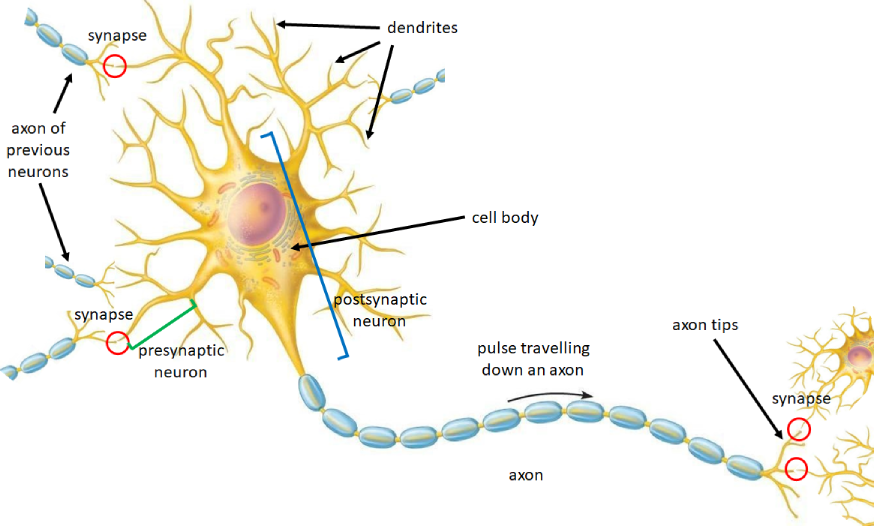
\includegraphics[width=0.8\linewidth]{Report-LateX-Template/fig/neuron.png}
	\caption{Basic model of a Neuron. source: Pearson Education Inc.}
	\label{fig:neuron}
\end{figure}

\begin{figure}
	\centering
	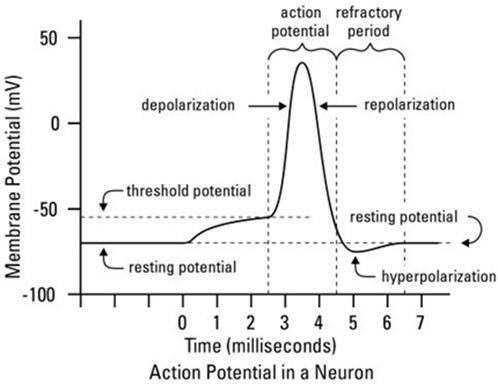
\includegraphics[width=0.5\linewidth]{Report-LateX-Template/fig/neuronactionpotential.png}
	\caption{Change in action potential of a neuron to a stimulus. source: Khan Academy}
	\label{fig:neuron2}
\end{figure}
 

\subsection{Other Neuromorphic Hardware}
\subsubsection{SpiNNaker}
University of Manchester's SpiNNaker project \cite{painkras2013spinnaker} is a microprocessor-based system optimized for real-time spiking neural networks. The main goal is to improve the performance of software simulations. It uses a custom fabricated chip that consists of 18 microprocessors in the size of 102 $mm^2$ using a 130 $nm$ process. It uses a fully digital architecture, which uses an asynchronous message passing network ($2-D$ torus) for interchip communication. In a 48-chip board configuration \cite{stromatias2013power}, consumes 25–36 W running at real-time while creating networks with hundreds of thousands of neurons and tens of millions of synapses.

\subsubsection{Intel Loihi}
Intel's Loihi \cite{8259423} is an in-house fabricated 60-$nm^2$ chip using 14-$nm$ process with on-chip learning capability. It is a rather new chip (2018) that has a wide range of new features such as hierarchical connectivity, dendritic compartments, synaptic delays, and programmable synaptic learning rules. It is demonstrated that Loihi running a custom version of Locally Competitive Algorithm, in the form of spiking convolutions can solve LASSO optimization problems with more than triple order of magnitude superior energy-delay-product when compared to conventional solvers running on a CPU iso-process/voltage/area. 
When compared to IBM's approach of developing neuromorphic chip, Intel joined the game in 2017 and quickly released it by 2018 for scientific purposes \cite{Tilley2017}. It provides some advantages over TrueNorth by offering on-chip training and testing, similar scalability and easy communication with non von Neumann devices. 


%\subsubsection{BrainChip}
%cite this article https://www.nextplatform.com/2018/09/11/first-wave-of-spiking-neural-network-hardware-hits/ 
%\begin{table}
%	\centering
%	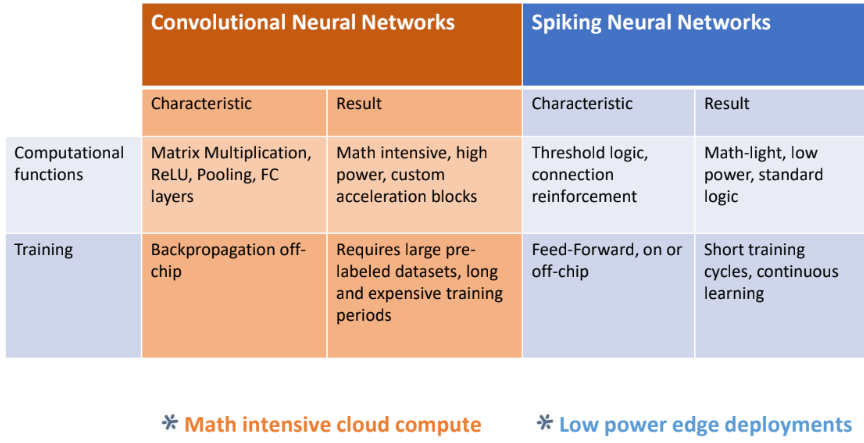
\includegraphics[width=0.8\linewidth]{Report-LateX-Template/fig/Brainchip.png}
%	\caption{BrainChip}
%	\label{fig:BrainChip}
%\end{table}

\section{IBM TrueNorth}
\label{sec:TrueNorth}

\begin{figure}
	\centering
	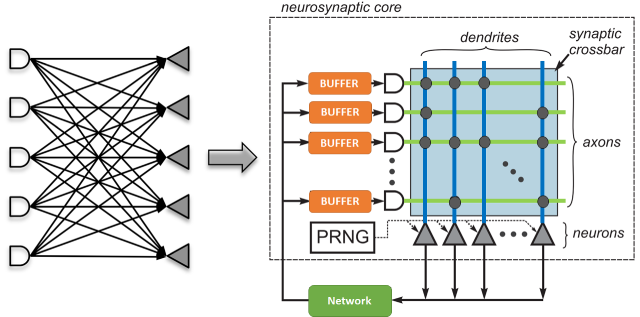
\includegraphics[width=0.5\linewidth]{Report-LateX-Template/fig/truenorthcore.png}
	\caption{Logical Representation of a TrueNorth core for a bipartite graph of a neural network. (as in Fig. 2 \cite{akopyan2015truenorth})}
	\label{fig:truenlogic}
\end{figure}

\subsection{Architecture \& Working}
The architecture of TrueNorth is a non von Neumann architecture, which does not use the traditional method of mapping instructions, into a linear memory with sequential programs. Instead, spiking neuron compute units are connected through a fast and efficient network which is covered in the previous section. During the initialization of the TrueNorth chip, the type of network should be specified and neuron behavior should be defined explicitly. Neurons are designed to use spikes for communicating with each other, mimicking the way brain works. Information is encoded using the frequency, time, and spacial distribution of spikes. From the Figure \ref{fig:neuron2}, x-axis represents time in milliseconds and y-axis represents membrane potential in milliVolts. Frequency of spikes, time they arrive, and spacial distribution can be modulated, and thereby action potential can be varied for each neuron. Figure \ref{fig:truenlogic} depicts a single neurosynaptic core that can have a maximum of 256 neurons and up to 64000 programmable synapses. 4096 neurosynaptic cores are arranged in a 64x64 two dimensional grid pattern in a single TrueNorth chip. In total, a TrueNorth chip has 1,048,576 neurons with over 268 million programmable synapses. TrueNorth chip is designed in such a way that, multiple TrueNorth chips can be used in different grid configurations depending on the computational power needed. Asynchronous circuits operate independently without a clock signal where as, synchronous circuits operate with a global clock signal. TrueNorth chip is a hybrid example of both circuits where, each neurosynaptic core has it's individual synchronization signal, and overall chip cores communicate through a network asynchronously, with a 1-bit 4-phase handshake protocol proposed by Muller \textit{et al.}\cite{muller1956theory}. From the Fig. \ref{fig:onebit}, to send a value "0", "data 0" line is set to High state (arrow 1) by sender, acknowledgement line is set to high (arrow 2) by receiver until transmission is completed by setting data 0 and ack to Low state (arrow 3 followed by arrow 4). To send value "1" again the whole process is repeated for "data 1". This asynchronous circuit is called a quasi delay-insensitive (QDI) circuit, which minimizes the number of interface signals between the cores. QDI asychronous piplines enable communication in between multiple TrueNorth chips like a single chip with many cores.This reduces the active and static power consumption of TrueNorth chip, by enabling high speed operation in real time as they are event-driven circuits.


\begin{figure}
	\centering
	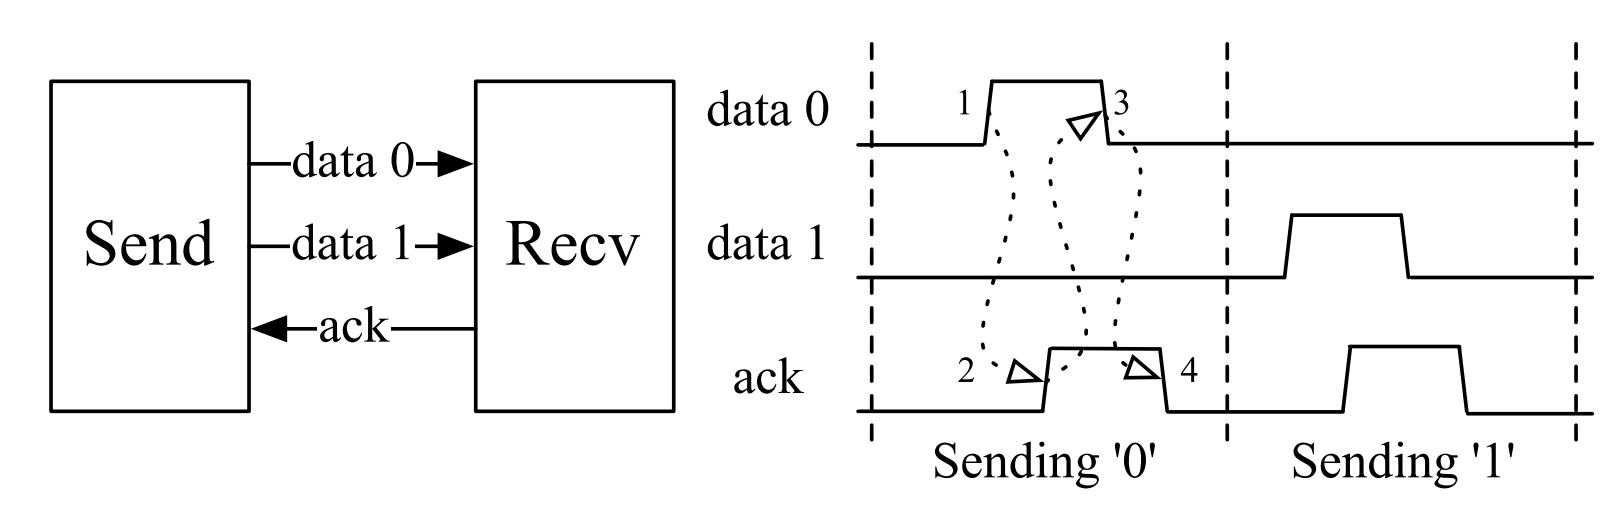
\includegraphics[width=0.4\linewidth]{Report-LateX-Template/fig/onebit.PNG}
	\caption{Asynchronous 1-bit 4-phase handshake.}
	\label{fig:onebit}
\end{figure}

\textbf{Neurosynaptic Core Construction:} It consists of input buffers, axons (represented by horizontal green lines), dendrites (represented by vertical blue lines), and neurons (represented by triangles). Axons and dendrites are connected by synapse (represented by a black dot). When the spikes arrive from the network, neurosynaptic core stores them in input buffers. A 1000 Hz synchronization signal called tick is generated in the core, the spikes from input buffers are distributed across the corresponding axons for that specific tick. If there is a synaptic connection between an axon and a dendrite, the spike travels to the connected neuron through dendrite. All incoming spikes are integrated into a neuron and membrane potential is updated. The leak value is subtracted from the membrane potential afterward. If the membrane potential exceeds the action potential, the generation of spike happens and sent into the network. A specific axon is located in the same core or in a different core depending on the configuration of neural network. All the computations for the current tick should complete before the next tick arrives and the duration is 1 ms.
\par
Simplified equation for calculating the membrane potential $V_j(t)$ of the $j$th neuron at tick $t$ is:
\centerline{$V_j(t) = V_j(t-1) + \Sigma_{i=0}^{255}A_i(t)w_{i,j}s_{j}^{G_i}-\lambda_j$}
\newline where $A_i(t)$ is an incoming spike on $i$th axon at time $t$, and $w_{i,j}$ is 1 if there is a connection between axon and dendrite, $w_{i,j}$ is 0 otherwise. $G_i$ value is an integer value from 1 to 4 used to specify the type of $i$th axon from four types. $\lambda_j \in \{ 0,1 \}$ is the leak used to reduce the noise. The role of input buffers is to accommodate communication delays in the network from different neurons or from neurons in different cores. Note that the values of leak and threshold should be correctly configured based on training phase of the NN model, and as they have significant impact on results as TrueNorth is only used for testing phase. Unfortunately, Akopyan \textit{et al.} \cite{akopyan2015truenorth} do not specify the types of axons, and which configuration to be used. A solution to this problem, is by experimenting with the provided tool and choose which type suits the model.

\textbf{Physical Layout:} The Fig. \ref{fig:physic} shows the physical construction of chip. The 2-D mesh network of multiple cores was made possible due to the intelligent design of the router. Router in every core communicates with 4 neighbouring cores in east, west, north, and south direction, along with internal communication in the core itself. Each spike arriving the router brings a relative $dx, dy$ address of a destination core, where $dx$ is the number of hops in the x direction and $dy$ is the number of hops in the y direction. A 9-bit signed integer is used to define the number of hops to find the destination core. It also contains parity flags, destination axon index and a destination tick at which it is to be integrated. If the designated spike reaches the destination router (represented as A), the additional bits are ripped off and only data is sent to the Scheduler (represented as B). Scheduler stores these spikes in Core SRAM (represented as C) until the execution of the tick. SRAM can store 256-bit entries for 16 ticks. 256 neurons in the core will always be scheduled till 16 ticks at any given point of time, if needed. All the spikes $A_i(t)$ are read by the scheduler for the current tick and passed on to token controller (represented by F). Token controller plays an vital role by controlling the neuron block execution. It computes the membrane potential using the above formula for all 256 neurons one-after-another. Synaptic connectivity $w_{i,j}$ is sent from the core SRAM to the token controller; meanwhile the other neuron parameters and current membrane potential are sent to the neuron block. If there is an active input spike ($A_i(t) = 1$) and associated synapse is active ($w_{i,j} = 1$), then only token controller sends a clock signal and an instruction about axon type $G_i$ to the neuron block. If either of them are not $1$, there is no event in the neuron block. Additionally after this process for all 256 neurons, token controller send instructions for neuron block for subtracting the leak $\lambda_j$ and for checking the spiking condition. If the new membrane potential $V_i(t) > threshold$, router receives a new spike packet from neuron block for sending it in the network. To mark the completion of the process for a single neuron, new and updated membrane potential is stored in the core SRAM. Token controller halts the computation by stopping the sending of clock pulses to neuron block. token controller send feedback to scheduler asking it to update its tick pointer to the next.

Due to physical limitation in the total number of I/O pins, merge-and-split blocks handle the communication between multiple TrueNorth chips with a custom peripheral circuitry. Author Akopyan \textit{et al.} \cite{akopyan2015truenorth} describes in depth about the Core internals of TrueNorth chip. 

\begin{figure}
	\centering
	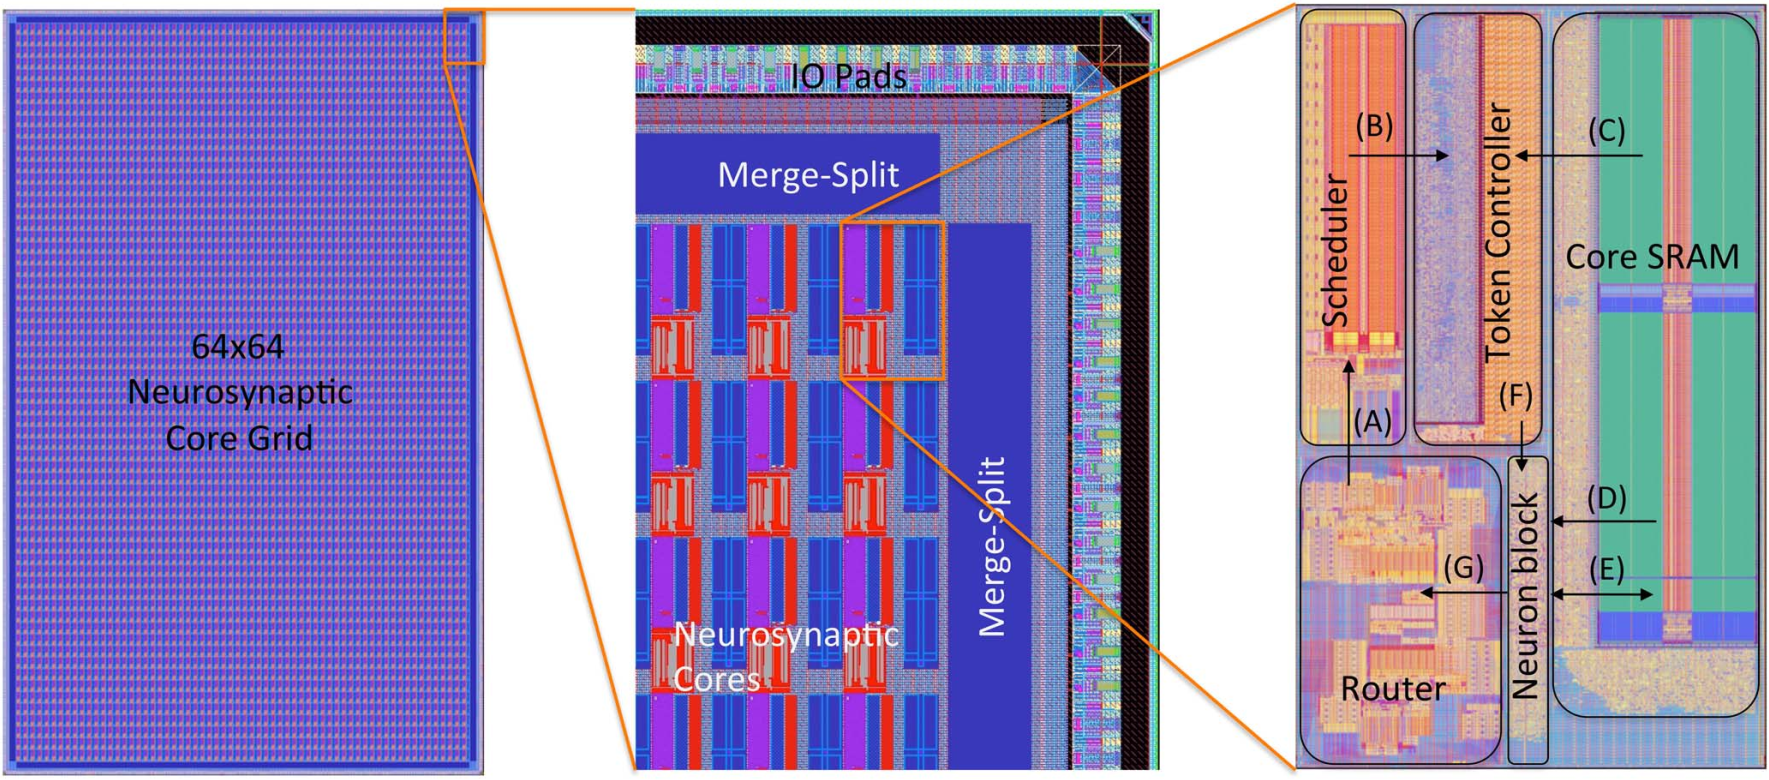
\includegraphics[width=0.8\linewidth]{Report-LateX-Template/fig/physic.PNG}
	\caption{Cross-section of a TrueNorth chip consisting of 4096 cores in 64x64 2-D grid. To the right shows a single core with a router, scheduler, token controller, core SRAM and neuron block (as in Fig. 5 \cite{akopyan2015truenorth})}
	\label{fig:physic}
\end{figure}

Figure \ref{fig:NS1e} shows the various configurations in which Trueorth chips are available. NS1e has single TrueNorth chips while, NS1e-16 has 16 such NS1e boards connected via a common Ethernet switch. NS16e is the latest configuration where 16 TrueNorth cores on a single board, thus the name "NS-(16)-e". This proves that it is scalable. Figure \ref{fig:tnarchi} shows the 3-level architecture of TrueNorth chip in the dimensions of Neuroscience, Structural, Functional and Physical over X axis and more detailed level over Y axis with Multi-Chip, Chip and core. This figure tell the whole evolution story of TrueNorth chip. As $C B A$ levels progress, a primate's brain was studied and a network was formed and each information is mapped on the brain and how the neuron works using canonical cortical microcircuit. Then Structural development was done based how the network must be designed from left to right $A D$; $B E$; $C F$. Similarly Functional design was done. $G$ shows the logical representation from figure \ref{fig:truenlogic}. $H$ represents the router configuration in a network between the cores. $I$ represents the connectivity between different TrueNorth chips. $J K L$ represent the physical core, Chips on the wafer and chip-to-chip connectivity respectively.


\begin{figure}
	\centering
	\includegraphics[width=0.6\linewidth]{Report-LateX-Template/fig/NS1e.png}
	\caption{NS1e, NS1e-16, NS16e compute modules from left to right depicting arrangement of 1, 16, 16 TrueNorth chips. source:www.elektroniknet.de}
	\label{fig:NS1e}
\end{figure}

\begin{figure}
	\centering
	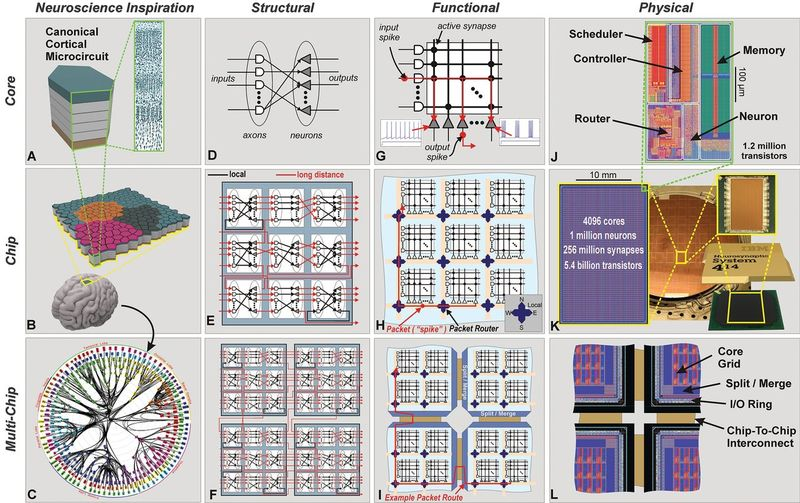
\includegraphics[width=1\linewidth]{Report-LateX-Template/fig/truenortharchitecture.png}
	\caption{TrueNorth 3-level Architecture. source:www.greencarcongress.com}
	\label{fig:tnarchi}
\end{figure}



\subsubsection{Compass: a TrueNorth Tool}
Along with a TrueNorth chip, IBM scientists Akopyan \textit{et al.} \cite{akopyan2015truenorth}, Preissl \textit{et al.} \cite{6468524} created a software tool that is an exact true replica of how TrueNorth works. This enabled them to cross-verify their designs and during the manufacturing process of the chip itself. They used Samsung’s 28 nm LPP CMOS process technology for silicon fabrication of TrueNorth chip as it is well suited for low-power devices. To further reduce power consumption of the chip, they used field-effect transistors with longer channel lengths. Since TrueNorth chip is larger than a typical ASIC chip in dimensions, manufacturing defects were taken into consideration during the design phase itself. High-yield manufacturing rules were followed during the physical design at mask level. With the help of the tool, testing and debugging was made easy as it is one-to-one equivalent. Even if some cores do not work due to defects, they can be easily isolated as it is an included advantage in using digital circuits over analog circuit for designing artificial neurons. 
Compass as tool uses custom language for communication called Corelet language. It can be used to simulate and train NN models irrespective whether you have the chip or not. It uses Corelet programming language which is domain specific and no available as open source. It also implements very large-scale integration (VLSI) placement tools for mapping logical neural networks to physical core locations on the TrueNorth chip. to achieve efficient run time operation. This happens during deployment phase. All the configurations for the network can be tested before deployment to achieve maximum accuracy. In future, this feature would be helpful for automakers to release on-the-air software updates for self driving cars. These software updates would be better trained models than previous generations. 

\subsection{Usage of TrueNorth chip}
\subsubsection{Self Driving Robot}
In 2017, Authors Hwu \textit{et al.} \cite{hwu2017self} built a self driving robot to show that TrueNorth is capable of assisting autonomous driving. In their experiment, IBM NS1e board was used along with Android-based robotics platform (see Figure \ref{fig:selfrobo}).  The robot utilises the built-in sensors of the android phone, and communicates with the Base Station for image processing, also with NS1e board for driving instructions in real-time. Base Station consists of, Penguin Server+Titan X GPUs for pre-processing of images and training the model. Trained custom TrueNorth model is send to NS1e board, for real-time testing and path prediction. Images taken in high resolution (176x144 RGB) are converted to 12 features (44x36) and sent to android phone. They are transduced into XYF spikes (where XYF mean X, Y and Forward directions) and sent via TCP connection to NS1e board. These XYF spikes are converted into TrueNorth spikes and with the help of TN API, TN core generates results which are again sent to android phone and converted into Class Histogram. Based on this, instructions are send to motor controller via Bluetooth to move in a specific direction. Output of TrueNorth classifier is shown in the Figure \ref{fig:selfrobo} and it successfully followed the hikers path shown from a satellite image. Results from this experiment show a decent improvement in the prediction accuracy with the increase in total core count \cite{hwu2017self}. This chip holds future for self driving battery cars as overall setup functioned on a Duratrax NiMH Onyx 7.2V 5000mAh battery, which is less than a fraction of typical consumption of a self driving car\cite{9007413}.


\begin{figure}
	\centering
	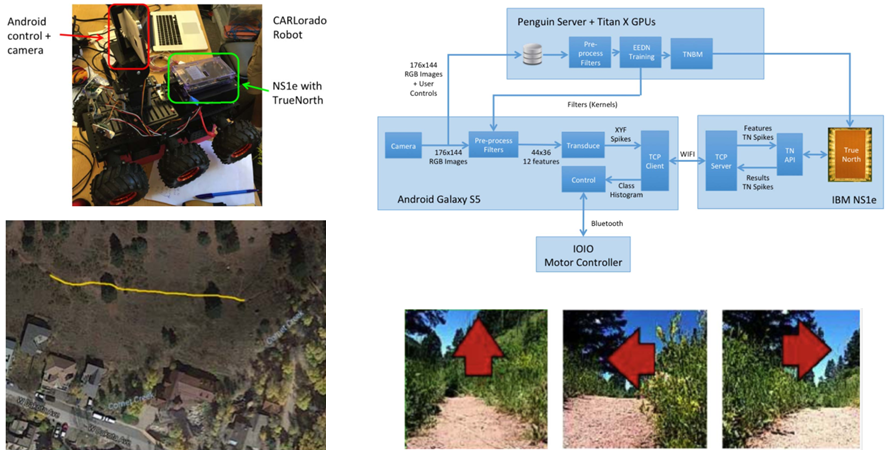
\includegraphics[width=0.8\linewidth]{Report-LateX-Template/fig/selfdrivingrobot.png}
	\caption{(in clockwise direction) Physical connection of TrueNorth NS1e and CARLorado; Data pipeline for running CNN; TrueNorth Classifier Prediction; Mountain trail in Telluride, Colorado (as in Figures 5,7,8,9 \cite{hwu2017self})}
	\label{fig:selfrobo}
\end{figure}

\subsubsection{Pharmaceutical and Bioinformatics Applications}
In 2016, Pastur \textit{et al.} \cite{pastur2016deep}, present a survey about the usage of different types of Deep Neural Networks (DNNs) in Medical Industry and how neuromorphic chips will revolutionize further advancements. They cover the following application areas: drug design, virtual screening (VS), Quantitative Structure–Activity Relationship (QSAR) research, protein structure prediction and genomics (and other omics) data mining. In these areas, DNN models were perfected over the decades, and good training, testing datasets are available for standardising the newer methods and models. They emphasise on the future need of neuromorphic hardware for DNNs. IBM TrueNorth and SpiNNaker chips were reviewed, and reached a important conclusion that considering not only neurons, as DNNs and neuromorphic chips should also include glial cells, given the proven importance of astrocytes, a type of glial cell which contributes to information processing in the brain. Though glial cells do not spike like neurons but are responsible for maintaining synaptic connections between neurons. This functionality will be useful for designing brain implants for patients with loss of motor abilities, etc. Authors suggest that, the Deep Artificial Neuron–Astrocyte Networks (DANAN) could overcome the difficulties in architecture design, learning process and scalability of the current ML methods. They strongly suggest major companies like Google, Facebook, Microsoft, Apple and IBM to focus their research on this neuromorphic hardware. Due to lack of supporting hardware and community support, the field of Cognitive/Neuromorphic Computing is unable to grow.


%\subsubsection{2015: Solving the incompatibility between backpropagation and neuromorphic hardware}
%Esser \textit{et al.} \cite{esser2015backpropagation}, predominantly show the incompatibility between backpropagation and neuromorphic hardware, and present a learning rule and a network topology that bridges the gap. The essence of the learning rule is to train a network offline with hardware supported connectivity, as well as continuous valued input, neuron output, and synaptic weights, but values constrained to the range $[0; 1]$. Further, such constrained values represent probabilities, either of a spike occurring or of a particular synapse being on.Such a network can be trained using backpropagation, but also has a direct representation in the spiking, low synaptic precision deployment system, thereby bridging these two worlds. The network topology uses a progressive mixing approach, where each neuron has access to a limited set of inputs from the previous layer, but sources are chosen such that neurons in successive layers have access to progressively more network input.

%In their novel approach:
%\begin{compactenum}
 %   \item they demonstrated for the first time an offline training methodology using backpropagation to create a network that employs spiking neurons, synapses requiring less bits of precision than even trinary weights, and constrained connectivity,
  %  \item they achieved the best accuracy to date (as of 2015) on MNIST (99:42\%) when compared to networks that use spiking neurons, even with high precision synapses (99:12\%), as well as networks that use binary synapses and neurons (97:88\%),
   % \item they demonstrate the network running in real-time on the TrueNorth chip, achieving by far the best published power efficiency for digit recognition (4 $\mu$J per classification at 95\% accuracy running 1000 images per second) compared to other low power approaches (6 mJ per classification at 95\% accuracy running 50 images per second).
%\end{compactenum}


%\subsubsection{2017 long short-term memory on a neurosynaptic processor}
%Shrestha \textit{et al.} \cite{shrestha2017spike}, present a limitation of TrueNorth when applied on temporal sequence processing models such as recurrent neural networks (RNNs). The reasons include, hardware constraints in connectivity and synaptic weight resolution, and the inherent difficulty in capturing temporal dynamics of an RNN using spiking neurons. They present a design flow that overcomes these difficulties and selected Long Short-Term Memory (LSTM) to map onto a spike based computation. They present a framework built on various approximation techniques, weight and activation discretization, spiking neuron sub-circuits that implements the complex gating mechanisms and a store-and-release technique to enable neuron synchronization and faithful storage. Two benchmark LSTM applications, parity check and Extended Reber Grammar, were evaluated and their accuracy, energy and speed trade-offs were analyzed. They divided standard LSTM is divided into modules and separately approximated using spiking neurons. On TrueNorth, modules are in the form of corelets which are then combined, connected and mapped to form Spike-based LSTM networks and synchronized using a store-and-release mechanism. When these networks were tested on two RNN benchmarks, they achieved results with promising accuracy and high power efficiency.

\subsection{Pros and Cons}
Some Pros of using TrueNorth chip include the following:
\begin{itemize}
  \item Having memory and processing at a single place reduces the power consumption.\cite{akopyan2015truenorth, hwu2017self, mead1990neuromorphic, indiveri2011neuromorphic} 
  \item Significantly increased efficiency for pre-trained models. \cite{akopyan2015truenorth, pastur2016deep}
  \item Easy configurability of neurons.\cite{akopyan2015truenorth, hwu2017self} 
  \item Modular design to integrate any number of TrueNorth chips as a single chip.\cite{akopyan2015truenorth}
  \item Defects in the fabrication of silicon can be easily disabled. \cite{akopyan2015truenorth} 
  \item Compass tool enables to virtually test the NN model before deploying onto the chip. \cite{akopyan2015truenorth} 
\end{itemize}

\par
Some Cons of using TrueNorth chip include the following:
\begin{itemize}
  \item Interfacing with traditional devices is difficult. \cite{pastur2016deep, agarwal2015era} 
  \item Expensive technology and costly manufacturing process \cite{akopyan2015truenorth, agarwal2015era}
  \item Wide range of possible applications, but few supported hardware.\cite{agarwal2015era} 
  \item Memory limitation for complex CNNs with many hidden layers. \cite{diehl2016conversion} 
  \item Newer version of SNNs call for updated chip design. \cite{bellec2018long}
  \item Compass tool also has to run on traditional von Neumann device for training of the model, which will again be slow and depends on a GPU. \cite{agarwal2015era} 
\end{itemize}











\subsection{Future Challenges}
According the authors Agarwal \textit{et al.} \cite{agarwal2015era}, following are the challenges for a TrueNorth chip:

\begin{compactenum}
	\item With the growth of neural network, it induces delays in switching time of the network with which different cores communicate.
	\item The mesh of axons and dendrites are interconnected, due to leakage voltage/current at the neurosynaptic site, there is a chance of information not reaching the correct location.
	\item Predominantly Von Neumann devices will have problems while interfacing with the non- Von Neumann architecture chip.
	\item TrueNorth chips are costly and does not create an immediate demand for unconventional technologies.
	\item Most I/O devices are based on Von Neumann designs and there is need for an ecosystem of products that support this platform.
	\item There is a need for an alternative for SRAM. Then the need for an internal clock can be eliminated and made completely asynchronous.
	\item Maass \textit{et al.} \cite{DBLP:journals/corr/abs-1803-09574} in 2008 suggest a newer version of spiking neural networks that can handle Long Short Term Memory NNs, convolutional NNs and other hybrid neural networks which has been a limitation for TrueNorth chip as they need more memory.
\end{compactenum}


%cite this somewhere \cite{esser2016convolutional}

\section{Domain-Specific Architectures}
\label{sec:dsa}
In this section we would be discussing about the guidelines given by Patterson \cite{Hennessy_Patterson_2017} and whether TrueNorth chip follows them.
\begin{compactenum}
	\item \textit{Use dedicated memories to minimize distances of data movement.} \newline TrueNorth's memory and processing are not separated and work as a single computational unit. Therefore, data movement is most minimized. This obeys the guidelines but a newer factor has to be counted. There is another type of data movement, in the form of spikes using the on-chip internal router network. There is no enough evidence to prove that latency is non-existent; therefore, this guideline is not completely followed 
	\item \textit{Invest resources into more arithmetic units or bigger memories} \newline TrueNorth's individual cores utilize resources on the need basis and there is no sharing of resources or resource allocation. Hence this guideline is not followed. Even without following this guideline, it is achieving the desired overall optimised result.
	\item \textit{Use the easiest form of parallelism that matches the domain} \newline TrueNorth does not follow traditional MIMD, SIMD or VLIW architectures but achieves parallelism with a custom architecture design. Hence, this guideline is also not followed.
	\item \textit{Reduce data size and type to simplest needed for the domain} \newline TrueNorth does follow this guideline partially as it computes only small data size but the data is in the form of spikes and each core has it's own 16x256-bit optimized storage that never directly interacts with spike. It is the most simplest for needed for it's operation.  
	\item \textit{Use of Domain-specific programming language} \newline TrueNorth uses Corelet language that is specific to the domain. Hence, this guideline is followed. 
\end{compactenum}


%\section{Scrap data}
%TrueNorth was able to classify images at between 1,200 and 2,600 frames per second (fps), while drawing just 25 to 275 milliwatts of power. That works out to about 6000 fps per watt, which would allow a low-power device to classify images in real-time from dozens of standard TV video feeds simultaneously. For the sake of comparison, NVIDIA’s latest purpose-built inferencing GPU, the Tesla P4, can classify images at about 160 images per second per watt using AlexNet.

%Training the model was performed with conventional GPUs, using functions from the MatConvNet toolbox, along with some customizations. On the inferencing side, the researchers developed an algorithm that exploited the low precision synapses and spiking neuron design of the TrueNorth processor. For the demonstration, eight image and audio benchmarks were employed, using five configurations of 0.5, 1, 2, 4, or 8 of the chips.

%In retrospect, maybe it shouldn’t come as a surprise that a neuromorphic architecture would be so adept at neural networks. But at the time TrueNorth was developed in 2011, the modern approach to convolutional networks was just getting traction. So while there was no design consideration for such a model, it became apparent to the researchers that the underlying architecture was well-suited to the application model once the appropriate algorithm was devised.

%Beside embedded deep learning applications on smartphones, robots and such, a TrueNorth-accelerated system could also be the basis of a scalable approach for deep learning inferencing in hyperscale or HPC datacenters. A possible testbed for such research already exists at the Department of Energy’s Lawrence Livermore National Laboratory (LLNL). In March, the lab installed a 16-chip TrueNorth array, known as NS16e, which was designed to explore scalable neuromorphic computing.

%One of the applications LLNL is currently looking at is how to use the processor to identify cars from overhead imagery, like for example, from video captured by airborne drones. Another use case explores the detection of defects in additive manufacturing (industrial 3D printing). A third application area being researched is how to use the platform to supervise physics simulations in industrial designs.

%The deep learning demonstration indicates that the architecture has an even broader scope though, and one that dovetails nicely with commercial developments in AI. Says Modha: “This work finally proves that the neuromorphic approach can be efficiently used in real-world applications and has significant advantages over conventional digital devices when energy consumption is considered.”

\newpage
\section{Conclusion}
\label{sec:conclusion}
The aim of domain-specific architectures is to move away from general purpose architectures to more sophisticated architectures that are energy-efficient depending on the application domain. IBM as a team took an unconventional approach by creating a neuromorphic chip with non von Neumann architecture in a short period of 10 years. Traditional architectures over the time have proven that number of transistors could reach a physical limit and efficiency does not increase. This problem is solved by IBM's TrueNorth and Intel's Loihi by using a scalable architecture. Though practical uses are limited to a few, it will take few more years to find new uses. Most of the hardware being predominantly Von Neumann machines, there is a need for hardware ecosystem with non-Von Neumann devices that store data and compute at the same time.
With the non sequential approach introduced by IBM and immediately followed by Intel with their Loihi chip, this shows that, leading chip manufacturers will be investing more into cognitive computing in the near future. Though they are in a primitive stage as of now, coming generations of neuromorphic chips will be affordable as well. Until then, we must choose whichever hardware that suits our domain or start developing new solutions by borrowing ideas from the nature.
On a side note, after 2017, interest into TrueNorth chip has reduced. Affordability is the core reason for any long term existence of a technology. A smaller form factor version of TrueNorth should be made affordable in a commercially viable way. It will benefit IBM as there will be more application domains from individual creators. With the growing hobbyists like RaspberryPi community, everyone would be interested in talking about this new invention. This can revolutionize almost every possible industry as would is being driven by data.
Though TrueNorth shows a reliable example of High-throughput with low batch size with the self driving robot\cite{hwu2017self}, there is enough evidence to confirm that, it will give similar results with other experimental setups. Hopefully we will be seeing a world with successors of IBM TrueNorth and Intel Loihi.



\nocite{Hennessy_Patterson_2017}

\bibliography{Template-Report}
\bibliographystyle{plain}

\end{document}
